\documentclass[11pt,a4paper]{article}

% ---------------------------------------------------------------------------
% Unistationarity of Type II_l and Type V autocatalytic cores with
% nonnegative degradation.
%
% Author metadata: set the three macros below before submission.
% ---------------------------------------------------------------------------
\newcommand{\PaperAuthor}{}
\newcommand{\PaperAffiliation}{}
\newcommand{\PaperDate}{14 September 2026}

\usepackage[T1]{fontenc}
\usepackage[utf8]{inputenc}
\usepackage{lmodern}
\usepackage{microtype}
\usepackage[a4paper,margin=1.05in]{geometry}
\usepackage{amsmath,amssymb,amsthm,mathtools}
\usepackage{graphicx}
\usepackage{float}
\usepackage{booktabs}
\usepackage{array}
\usepackage{enumitem}
\usepackage{xcolor}
\usepackage{listings}
\usepackage[obeyspaces,spaces]{url}
\usepackage[colorlinks=true,linkcolor=blue!55!black,citecolor=blue!55!black,urlcolor=blue!55!black]{hyperref}

\hypersetup{pdftitle={Unistationarity of Type II and Type V autocatalytic cores with nonnegative degradation},
  pdfsubject={Uniqueness of positive stationary states for reversible diluted autocatalytic cores with mixed degradation},
  pdfkeywords={autocatalysis, autocatalytic cores, chemical reaction networks, mass action, unistationarity, degradation, implicit function theorem, Lean 4}}

\setlist{itemsep=2pt,topsep=3pt}
\setlength{\emergencystretch}{1.5em}

\lstdefinelanguage{Lean}{
  morekeywords={theorem,def,structure,inductive,namespace,end,import,by,intro,exact,constructor},
  sensitive=true,
  morecomment=[l]{--},
  morestring=[b]",
}
\lstset{
  language=Lean,
  basicstyle=\ttfamily\small,
  keywordstyle=\bfseries,
  commentstyle=\itshape\color{black!60},
  columns=fullflexible,
  keepspaces=true,
  breaklines=true,
  frame=single,
  framerule=0.3pt,
  xleftmargin=1em,
  xrightmargin=1em,
  extendedchars=true,
  literate={≤}{{$\le$}}1 {ℕ}{{$\mathbb{N}$}}1 {ℝ}{{$\mathbb{R}$}}1 {→}{{$\to$}}1 {∀}{{$\forall$}}1 {∃}{{$\exists$}}1 {≠}{{$\neq$}}1 {∧}{{$\wedge$}}1 {¬}{{$\neg$}}1
}

\theoremstyle{plain}
\newtheorem{theorem}{Theorem}[section]
\newtheorem{proposition}[theorem]{Proposition}
\newtheorem{lemma}[theorem]{Lemma}
\newtheorem{corollary}[theorem]{Corollary}
\theoremstyle{definition}
\newtheorem{definition}[theorem]{Definition}
\newtheorem{example}[theorem]{Example}
\theoremstyle{remark}
\newtheorem{remark}[theorem]{Remark}

\numberwithin{equation}{section}

\newcommand{\R}{\mathbb{R}}
\newcommand{\N}{\mathbb{N}}
\newcommand{\Z}{\mathbb{Z}}
\newcommand{\one}{\mathbf{1}}
\newcommand{\diag}{\operatorname{diag}}
\newcommand{\Ker}{\operatorname{ker}}
\newcommand{\II}{\mathrm{II}}
\newcommand{\V}{\mathrm{V}}
\newcommand{\Top}{\mathrm{(Top)}}
\DeclareUrlCommand\lean{\urlstyle{tt}}

\title{Unistationarity of Type $\II_\ell$ and Type $\V$ autocatalytic cores\\ with nonnegative degradation}
\author{\PaperAuthor\\ \PaperAffiliation}
\date{\PaperDate}

\begin{document}
\maketitle

\begin{abstract}
Nandan, Nghe and Unterberger classified the minimal autocatalytic cores of diluted reaction networks into five families and proved that, under strictly positive linear degradation of every species, every classified core has at most one positive stationary state, with the exception of the Type $\II_\ell$ cores with $\ell>2$ forks, which were settled subsequently. They asked whether uniqueness survives \emph{mixed} degradation, in which some species are degraded and others are not, and left this open for the Type $\V$ cores and the Type $\II_\ell$ cores with $\ell>2$. We answer both cases affirmatively. For the reversible mass-action extension of every source-minimal Type $\II_\ell$ core ($\ell\ge3$) and every source-minimal Type $\V$ core, with arbitrary positive forward and reverse rate constants and an arbitrary nonnegative degradation vector, there is at most one strictly positive stationary concentration vector; the conclusion includes every internal species of the unit paths permitted by the classification and does not assume that any degradation constant is positive. Combined with the published results for the remaining families, this gives unistationarity across the whole classification for all nonnegative degradation vectors. Two mechanisms are used. Exact elimination of passive reversible unit paths, which remains valid when internal losses vanish, reduces Type $\V$ to three polynomial equations whose coordinate ratios admit a strict extremum argument. For Type $\II_\ell$ a stationary-flow factorization of the Jacobian and an admissibility shift show that the stationary Jacobian is nonsingular at every positive stationary state, even on the boundary of the degradation orthant, by transporting the positive-degradation current criterion through the positive diagonal orthant with a multiaffine determinant argument; the implicit-function theorem then transfers uniqueness from positive degradation to its boundary. We also derive a quantitative lower bound $\det(-H)\ge(\det N)^2\prod_i\min(p_i,q_i)$ for the scaled stationary Jacobian, local smooth continuation of the positive state through vanishing loss coefficients, and existence and local asymptotic stability of the unique positive state for all sufficiently small nonnegative degradation. The two family uniqueness theorems and the algebraic kernel criteria are verified in Lean~4 against Mathlib with warnings treated as errors and no unproved declarations.
\end{abstract}

\noindent\textbf{Keywords.} autocatalysis; autocatalytic cores; chemical reaction networks; mass-action kinetics; unistationarity; degradation; implicit function theorem; formal verification.

\medskip
\noindent\textbf{MSC 2020.} 92C42, 80A30; secondary 15B48, 34C99, 68V20.

\section{Introduction}\label{sec:intro}

A reaction network is autocatalytic when a set of species can amplify itself from an external food supply. The question of which small motifs are capable of this, and how they behave dynamically, goes back to the autocatalytic sets of Kauffman~\cite{Kau86} and the reflexively autocatalytic food-generated sets of Hordijk and Steel~\cite{HS04}, and was given a stoichiometric foundation by Blokhuis, Lacoste and Nghe~\cite{BLN20}. In the \emph{diluted regime}, where every reaction consumes a single molecule of the autocatalytic species, Unterberger and Nghe~\cite{UN22} showed that stoichiometric autocatalysis is equivalent to a topological condition $\Top$ on the split graph of the network. Nandan, Nghe and Unterberger~\cite{NNU26} then classified the minimal networks satisfying $\Top$, the \emph{autocatalytic cores}, into five families, and studied the mass-action dynamics of their reversible extensions under linear degradation of every species.

Among the dynamical results of~\cite{NNU26} is a uniqueness theorem: if every species is degraded at a strictly positive linear rate, every classified core has at most one positive stationary state, with the possible exception of the Type $\II_\ell$ cores with more than two cyclically ordered forks. That exception was removed in the companion paper~\cite{TypeIIpos}, which also showed by exact examples that minimality cannot be dropped. In the remark following their Theorem~5.2, Nandan, Nghe and Unterberger raise the \emph{mixed} case, in which some species are degraded and others are not, and note that their continuation argument does not settle it for the Type $\V$ cores and for Type $\II_\ell$ with $\ell>2$. Mixed degradation is the physically generic situation in a compartment or a flow reactor: a species bound to a surface, sequestered in a complex, or simply chemically inert on the relevant time scale has no direct loss term, while its partners are washed out or hydrolysed. The question is whether \emph{selective} linear loss alone can create a second positive operating state inside a minimal autocatalytic motif.

This paper answers that question in the negative for both open families.

\begin{theorem}[Main theorem]\label{thm:main}
Let $G$ be a source-minimal diluted autocatalytic core of Type $\II_\ell$ with $\ell\ge3$, or of Type $\V$, in the classification of~\cite{NNU26}. Give every reaction of its reversible extension strictly positive forward and reverse mass-action rate constants, and give every species $X_i$ a linear degradation reaction $X_i\to\varnothing$ with rate constant $d_i\ge0$. If $x$ and $y$ are strictly positive stationary concentration vectors for these parameters, then $x=y$. The equality includes every internal species of the reversible unit paths permitted by the classification.
\end{theorem}

The degradation vector $d$ is arbitrary in the closed nonnegative orthant: every mixed support is covered, and so are the all-zero and the all-positive vectors. The theorem asserts uniqueness, not existence; it makes no claim about stability, permanence or global convergence, and none about networks in which a core is coupled to other reactions.

\begin{corollary}[The whole classification]\label{cor:classification}
Every reversible extension of a source-classified minimal diluted autocatalytic core of~\cite{NNU26}, with positive reversible rate constants and an arbitrary nonnegative linear degradation vector, has at most one strictly positive stationary state.
\end{corollary}

\begin{proof}
Theorem~\ref{thm:main} supplies Type $\II_\ell$ with $\ell\ge3$ and Type $\V$. For the remaining classified cases, uniqueness under every nonnegative degradation vector follows from the undegraded and degraded results of~\cite{NNU26} (Theorems~4.1 and~5.2 and the remark following Theorem~5.2). The corollary is a conventional consequence of the cited statements; the present paper formalizes only the two families of Theorem~\ref{thm:main}.
\end{proof}

\subsection*{Why the positive-degradation arguments do not extend}
The proofs available for strictly positive degradation all divide by the degradation flux $e_i=d_ix_i$ of some species. The concentration-recovery formulas used in~\cite{NNU26} for Type $\V$ have a denominator that vanishes for a pair of species without degradation, and the current-kernel matrix $K=I-AE^{-1}N$ of~\cite{TypeIIpos} is built from $E^{-1}=\diag(e)^{-1}$. When a coordinate of $d$ vanishes, these objects do not merely become large; they cease to exist, and the estimates that rest on them lose the strict inequalities that force two stationary states to coincide. A naive limit $d_i\downarrow0$ is not available either, since uniqueness is not a closed condition. The mixed case therefore requires an argument that never divides by a loss coefficient.

\subsection*{The two mechanisms}
For Type $\V$ we give a direct proof. The classification permits each of the three pairs $(U_i,S_i)$ of a Type $\V$ core to be joined by an arbitrary finite reversible unit path or to be identified, giving eight combinatorial variants and unboundedly many networks. Lemma~\ref{lem:path} shows that a reversible unit path with nonnegative internal losses is exactly equivalent, at stationarity, to a single reversible reaction together with two nonnegative endpoint leakage terms, and that this remains true when every internal loss is zero. After elimination of the three fork sources, the stationary problem collapses to three polynomial equations in the three base concentrations $U_0,U_1,U_2$ with a uniform sign structure (Section~\ref{sec:typev}). Two positive solutions of such a system have three coordinate ratios, and a short extremum argument on the ratio of median sign shows that all three equal one. Strictness comes from the reverse fork kinetics, not from degradation, which is why zero loss coefficients are harmless.

For Type $\II_\ell$ the direct comparison of two states does not close, and we use a different strategy: we prove that every positive stationary state has a nonsingular Jacobian, even at boundary degradation, and then transfer uniqueness from positive degradation by the implicit-function theorem. The nonsingularity proof has three ingredients. First, the scaled stationary Jacobian $H$ has the exact factorization $-H=N(\diag(q)-B(e))N^{\mathsf T}$ in terms of the reverse flows $q$ and the degradation fluxes $e$, where $N$ is the invertible source stoichiometric matrix (Section~\ref{sec:boundary}). Second, the admissible reverse flows at fixed $e$ are exactly the translates $q=s(e)+t$, $t>0$, of a fixed \emph{admissibility shift} $s(e)=\max(0,-N^{-1}e)$, so interior nonsingularity for all admissible flows is the statement that $\det(A(e)+\diag(t))\neq0$ on the whole positive diagonal orthant. Third, a fixed matrix whose diagonal shifts are all nonsingular on the positive orthant has positive determinants there, this passes to nonnegativity in the limit $e\to\partial\R^n_{\ge0}$, and a multiaffine interpolation upgrades nonnegativity back to strict positivity (Lemmas~\ref{lem:orientation} and~\ref{lem:strict}). The interior input is the positive-degradation current criterion of~\cite{TypeIIpos}, which we restate in Section~\ref{sec:interior} in the form actually needed: its estimates use one stationary state only, and therefore prove nonsingularity of the Jacobian at every admissible positive flow, not only uniqueness.

\subsection*{Consequences}
The determinant argument has a quantitative form: every principal minor of $A(e)$ is nonnegative, and hence
\[
\det(-H)\ \ge\ (\det N)^2\prod_i\min(p_i,q_i)\ >0
\]
at every positive stationary state of a separated Type $\II_\ell$ skeleton, for every $e\ge0$ (Section~\ref{sec:consequences}). Nonsingularity gives locally smooth continuation of the positive stationary state through vanishing loss coefficients, so that turning an individual degradation constant through zero cannot produce a saddle-node between two positive states. At zero degradation the reversible core is detailed balanced with a unique positive state whose Jacobian is similar to a symmetric negative-definite matrix; by openness of the Hurwitz condition, every sufficiently small nonnegative degradation vector admits exactly one positive stationary state, and it is locally asymptotically stable. Finally, a nonnegative stationary state of any reversible core extension is either the origin or strictly positive.

\subsection*{Formal verification}
The two family statements of Theorem~\ref{thm:main} are compiled in Lean~4~\cite{dMU21} against Mathlib~\cite{mathlib20}, as an independent conjunction of two universal statements over the literal source normal forms, with no analytic object in the public interface (Section~\ref{sec:formal}). The algebraic three-ratio and tangent-kernel criteria for Type $\V$ and the general diagonal-orthant determinant lemmas are also formal. The consequences of Section~\ref{sec:consequences} and the identification of the source normal forms with the published classification are conventional mathematics and are labelled as such.

\subsection*{Organization}
Section~\ref{sec:setting} fixes the stationary problem and the two source normal forms. Section~\ref{sec:chains} proves the passive-path reduction. Section~\ref{sec:typev} proves the Type $\V$ case. Sections~\ref{sec:interior}--\ref{sec:finish} prove the Type $\II_\ell$ case: the interior current criterion, the boundary nonsingularity theorem, and the uniqueness transfer together with the coincident three-fork branch. Section~\ref{sec:consequences} collects the consequences, Section~\ref{sec:formal} documents the formal verification, and Section~\ref{sec:discussion} relates the result to injectivity criteria and lists open questions.

\section{The stationary problem and the source normal forms}\label{sec:setting}

\subsection{Diluted cores and their reversible extensions}
A diluted network on a species set $\{X_1,\dots,X_n\}$ is a set of reactions each consuming exactly one molecule of one species. Its \emph{split graph} has an edge $X_r\to X_i$ whenever some reaction consumes $X_r$ and produces $X_i$. The network is stoichiometrically autocatalytic when some nonnegative flux vector has strictly positive net production of every species; by~\cite{UN22} this is equivalent to $\Top$, the existence of a strongly connected component of the split graph containing a reaction with at least two products in the component. An \emph{autocatalytic core} is a network satisfying $\Top$ that is minimal under chemostatting, that is, under removal of species from the autocatalytic set together with the reactions that then lose their internal reactant~\cite[\S2]{NNU26}. The classification theorem of~\cite{NNU26} (their Theorem~3.1) lists five families of cores. Two of them concern us: the Type $\II_\ell$ cores, a main cycle carrying $\ell$ cyclically ordered fork reactions each of which produces its cycle successor with an integer multiplicity and one earlier species of the cycle with coefficient one, and the Type $\V$ cores, three pairs of species arranged so that each pair's fork produces one member of each of the other two pairs.

The dynamics studied in~\cite{NNU26} and here is the mass-action dynamics of the \emph{reversible extension}: every reaction is made reversible with strictly positive forward and reverse rate constants, and every species is given a linear degradation reaction. ``Diluted'' therefore describes the class from which the core is taken; the reverse reactions are nonlinear and are present in the dynamics.

\subsection{Stationary equations and flows}
Index the forward reactions of the core by their unique reactant, so that reaction $r$ consumes $X_r$. Let $P_{ir}\in\N$ be the number of molecules of $X_i$ produced by reaction $r$, and put $N=P-I$. With forward and reverse rate constants $a_r,b_r>0$ and degradation constants $d_i\ge0$, the species-formation rate is
\begin{equation}\label{eq:model}
p_r(x)=a_rx_r,\qquad q_r(x)=b_r\prod_ix_i^{P_{ir}},\qquad
f(x)=N\bigl(p(x)-q(x)\bigr)-\diag(d)\,x .
\end{equation}
All inequalities between vectors are coordinatewise. At a positive stationary state $x$ write
\begin{equation}\label{eq:flows}
p=p(x),\qquad q=q(x),\qquad J=p-q,\qquad e=\diag(d)\,x,\qquad NJ=e .
\end{equation}
The flows $p,q$ are strictly positive even when some coordinates of $e$ vanish; the currents $J_r$ may have either sign. When the network contains unit paths, their internal species carry their own balance equations, which are part of the stationary system; Section~\ref{sec:chains} eliminates them exactly.

\subsection{The Type \texorpdfstring{$\II_\ell$}{II\_l} normal form}\label{subsec:typeii}
Write $F_j$, $j\in\Z/\ell\Z$, for the fork sources in cyclic order. In the \emph{separated} form, the retained source species lie on a directed cycle with successor permutation $\sigma$, and every reaction has one of the two forms
\begin{equation}\label{eq:ii}
X_r\rightleftharpoons m_rX_{\sigma(r)}
\qquad\text{or}\qquad
X_r\rightleftharpoons m_rX_{\sigma(r)}+X_{\tau(r)},\qquad m_r\in\N_{\ge1},
\end{equation}
the second occurring exactly at the $\ell$ forks. Between consecutive forks $F_j$ and $F_{j+1}$ the cycle passes through a nonempty \emph{gap} of nonfork species; the last species $T_{j+1}$ of that gap is the back target $\tau(F_{j+1})$ of the following fork, and the reaction $T_{j+1}\to F_{j+1}$ has unit weight. Before contraction, the link from $T_{j+1}$ to $F_{j+1}$ is an arbitrary finite reversible \emph{return path} of one-to-one reactions with positive integer multipliers; the classification also allows the weak-order coincidence in which the stem leaving a fork has no separated nonfork vertex before the next fork. Figure~\ref{fig:normal} shows one period of the separated form.

Two consequences of source minimality rigidify this picture. They are proved in~\cite[Lemmas~3.1 and~3.2]{TypeIIpos}; we recall the statements and the ideas, because they determine exactly which networks Theorem~\ref{thm:main} covers.

\begin{lemma}[Source dichotomy]\label{lem:exhaustion}
Let $\ell\ge3$. A source-minimal Type $\II_\ell$ core is either fully separated, or $\ell=3$ and all three stems are coincident, in which case the core is the three-species network
\begin{equation}\label{eq:coincident}
X_i\rightleftharpoons m_iX_{i+1}+X_{i+2},\qquad i\in\Z/3\Z,\quad m_i\ge1 .
\end{equation}
\end{lemma}

\begin{proof}[Idea of proof]
If the stem leaving $F_j$ is coincident, retain the three species $F_j$, $F_{j+1}$ and the back target of $F_j$ and chemostat all others. The restricted split graph is strongly connected and the reaction at $F_j$ keeps two internal products, so the restriction satisfies $\Top$. It is proper unless the core has exactly these three species, which happens only when $\ell=3$ and every stem is coincident.
\end{proof}

\begin{lemma}[Unit return paths]\label{lem:unit}
In a separated source-minimal Type $\II_\ell$ core every stoichiometric multiplier on every return path equals one.
\end{lemma}

\begin{proof}[Idea of proof]
A return path from $T_j$ to $F_j$ closes into a directed cycle with the coefficient-one back product of $F_j$. If some multiplier on this cycle is at least two, an explicit positive flux, rotated so that the gain edge comes first, has strictly positive net production at every vertex of the cycle. The cycle is then a proper stoichiometrically autocatalytic restriction, contradicting minimality.
\end{proof}

Lemma~\ref{lem:unit} is applied only to return paths. An active reaction $X\rightleftharpoons mY$ with $m>1$ on the main cycle is never replaced by a linear path; all active integer weights of~\eqref{eq:ii} remain in the model throughout. The coincident case~\eqref{eq:coincident} is treated separately in Section~\ref{sec:finish}.

\subsection{The Type \texorpdfstring{$\V$}{V} normal form}\label{subsec:typev}
A Type $\V$ core consists of three pairs $(U_i,S_i)$, $i\in\Z/3\Z$. Within each pair there is a finite reversible unit path from $U_i$ to $S_i$, and at $S_i$ there is a fork
\begin{equation}\label{eq:v}
S_i\rightleftharpoons U_{i+1}+U_{i+2}.
\end{equation}
Each pair may instead be \emph{collapsed}, $U_i=S_i$, independently of the other two, so that the fork is $U_i\rightleftharpoons U_{i+1}+U_{i+2}$. This gives the eight identification patterns of the classification, with arbitrary finite unit paths in the linked pairs. In the notation of~\cite{NNU26} one may take $(U_0,U_1,U_2)=(u,x,x')$ and $(S_0,S_1,S_2)=(v,w,w')$. Every species, including every internal path species, may carry its own nonnegative degradation constant.

\begin{figure}[t]
\centering
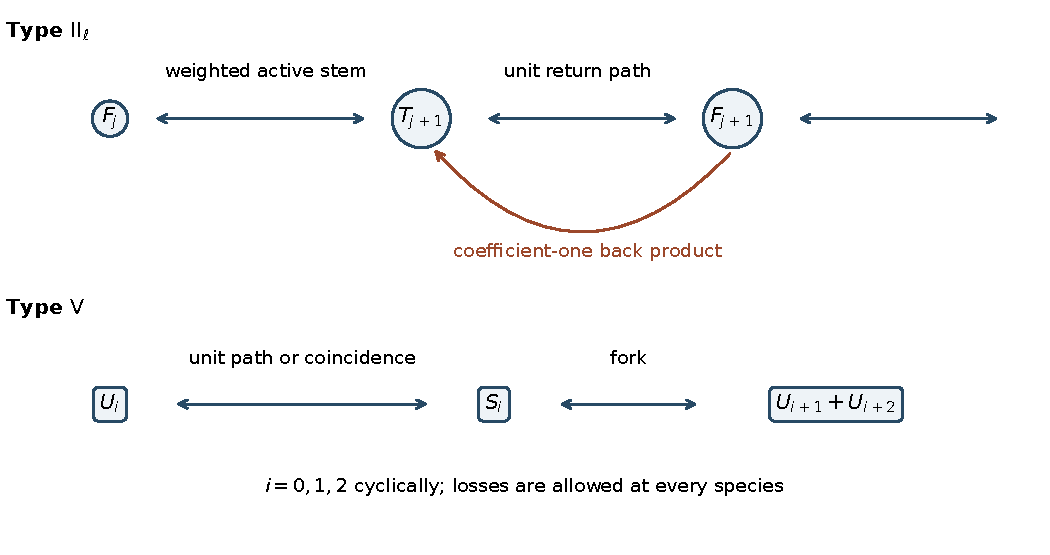
\includegraphics[width=.96\linewidth]{figures/normal_forms.pdf}
\caption{The two normal forms. In the Type $\II_\ell$ period, the active stem from $F_j$ to $T_{j+1}$ carries arbitrary positive integer weights and the return path from $T_{j+1}$ to $F_{j+1}$ is a reversible unit path; the coefficient-one back product of the fork $F_{j+1}$ returns to $T_{j+1}$. In Type $\V$ each pair is joined by a reversible unit path or collapsed, and each fork produces one member of each other pair. Arrows indicate the split graph. Every species may be degraded at a nonnegative linear rate.}
\label{fig:normal}
\end{figure}

\section{Exact elimination of passive paths}\label{sec:chains}

A reversible unit path consists of species $Z_0=X,Z_1,\dots,Z_m,Z_{m+1}=Y$ joined by reactions $Z_k\rightleftharpoons Z_{k+1}$ with rate constants $a_k,b_k>0$, and internal degradation constants $d_k\ge0$ at $Z_1,\dots,Z_m$. Write $j_L$ for the current leaving $X$ into the path and $j_R$ for the current entering $Y$ from it.

\begin{lemma}[Passive path reduction]\label{lem:path}
For every finite reversible unit path with positive rate constants and nonnegative internal degradation there are constants $c,\beta>0$ and $\lambda_L,\lambda_R\ge0$, depending only on the path parameters, such that every stationary internal state satisfies
\begin{equation}\label{eq:chain}
j_L=(c+\lambda_L)X-\beta Y,\qquad j_R=cX-(\beta+\lambda_R)Y .
\end{equation}
For fixed endpoint concentrations $X,Y$ the stationary internal concentrations are unique.
\end{lemma}

\begin{proof}
For a single edge, $j_L=j_R=a_0X-b_0Y$, so $(c,\beta,\lambda_L,\lambda_R)=(a_0,b_0,0,0)$. Suppose the path up to $Z$ has been reduced with parameters $(c,\beta,\lambda_L,\lambda_R)$, and append the edge $Z\rightleftharpoons Y$ with constants $a,b>0$ and loss $d\ge0$ at $Z$. The balance at $Z$ reads $j_R-(aZ-bY)-dZ=0$, that is,
\[
LZ=cX+bY,\qquad L=\beta+\lambda_R+a+d>0 .
\]
Substituting $Z=(cX+bY)/L$ into $aZ-bY$ and into the old $j_L$ gives~\eqref{eq:chain} for the extended path with
\begin{equation}\label{eq:pathrecursion}
c'=\frac{ca}{L},\qquad \beta'=\frac{\beta b}{L},\qquad
\lambda_L'=\lambda_L+\frac{c(\lambda_R+d)}{L},\qquad
\lambda_R'=\frac{b(\lambda_R+d)}{L},
\end{equation}
which have the asserted signs. The same substitution determines $Z$ uniquely from $X,Y$; the induction then determines every earlier internal concentration.
\end{proof}

At the endpoints,~\eqref{eq:chain} is a single reversible unit reaction with transmission constants $c,\beta$ together with two additional nonnegative linear losses, $\lambda_LX$ at $X$ and $\lambda_RY$ at $Y$. Hence compression preserves the form of the stationary equations: a Type $\V$ core with paths is, at stationarity, exactly the collapsed skeleton with modified rate constants and increased nonnegative endpoint losses, and similarly for the return paths of Type $\II_\ell$. Two features matter for the mixed case. The pivots $L$ are positive because of the reverse rate $a$ of the appended edge, not because of degradation, so the reduction is valid when every internal loss vanishes. And loss confined to an internal species is retained as effective endpoint leakage rather than lost: for $X\rightleftharpoons Z\rightleftharpoons Y$ with all four edge constants equal to one and $d_Z=1$, $d_X=d_Y=0$, one finds $c=\beta=\lambda_L=\lambda_R=1/3$.

\section{A three-variable proof for Type V}\label{sec:typev}

\subsection{Reduction to the base concentrations}
Apply Lemma~\ref{lem:path} to the path of each linked pair and absorb the endpoint leakage into the endpoint losses. For a linked pair $i$ let $a_i,b_i>0$ be the transmissions of its path, $f_i,g_i>0$ the forward and reverse constants of its fork~\eqref{eq:v}, and $d_i,h_i\ge0$ the total losses at $U_i$ and $S_i$ (degradation plus path leakage). Put $W_i=U_{i+1}U_{i+2}$. The stationary balance at $S_i$ is $a_iU_i-b_iS_i-(f_iS_i-g_iW_i)-h_iS_i=0$, so
\begin{equation}\label{eq:S}
S_i=\frac{a_iU_i+g_iW_i}{D_i},\qquad D_i=b_i+f_i+h_i>0 .
\end{equation}
The fork current $\delta_i=f_iS_i-g_iW_i$ and the total loss $L_i=d_iU_i+h_iS_i$ of the pair become
\begin{equation}\label{eq:response}
\delta_i=\alpha_iU_i-\beta_iW_i,\qquad L_i=\lambda_iU_i+\mu_iW_i,
\end{equation}
with
\[
\alpha_i=\frac{f_ia_i}{D_i}>0,\qquad
\beta_i=\frac{g_i(b_i+h_i)}{D_i}>0,\qquad
\lambda_i=d_i+\frac{h_ia_i}{D_i}\ge0,\qquad
\mu_i=\frac{h_ig_i}{D_i}\ge0 .
\]
For a collapsed pair the same representation holds with $(\alpha_i,\beta_i,\lambda_i,\mu_i)=(f_i,g_i,d_i,0)$. The essential point is the uniform sign structure: $\beta_i>0$ because the reverse fork constant $g_i$ is positive, regardless of the losses.

The species $U_i$ is produced by the forks of pairs $i+1$ and $i+2$ and consumed by its own pair; adding the balances at $U_i$ and $S_i$ gives the pair balance $\delta_{i+1}+\delta_{i+2}-\delta_i=L_i$. Adding the pair balances at $i+1$ and $i+2$ yields $2\delta_i=L_{i+1}+L_{i+2}$, hence
\begin{equation}\label{eq:reduced}
2\alpha_iU_i
=2\beta_iU_{i+1}U_{i+2}
+\lambda_{i+1}U_{i+1}+\lambda_{i+2}U_{i+2}
+\mu_{i+1}U_iU_{i+2}+\mu_{i+2}U_iU_{i+1},
\qquad i\in\Z/3\Z .
\end{equation}
Conversely, a positive solution of~\eqref{eq:reduced} determines $S_i$ by~\eqref{eq:S} and every internal path concentration by Lemma~\ref{lem:path}.

\subsection{The three-ratio lemma}

\begin{lemma}[Three ratios]\label{lem:ratios}
Let $A_i,B_i>0$ and $C_i,D_i,H_i,K_i\ge0$ for $i\in\Z/3\Z$. The system
\begin{equation}\label{eq:ratiosystem}
A_iu_i=B_iu_{i+1}u_{i+2}+C_iu_{i+1}+D_iu_{i+2}+H_iu_iu_{i+2}+K_iu_iu_{i+1}
\end{equation}
has at most one solution $u\in\R^3_{>0}$.
\end{lemma}

\begin{proof}
Let $u,v>0$ be solutions and $r_i=u_i/v_i$. Subtracting $r_i$ times the equation for $v$ from the equation for $u$ removes the left-hand side and gives, for each $i$,
\begin{equation}\label{eq:rowdefect}
\begin{aligned}
0={}&B_iv_{i+1}v_{i+2}\,(r_{i+1}r_{i+2}-r_i)
+C_iv_{i+1}(r_{i+1}-r_i)+D_iv_{i+2}(r_{i+2}-r_i)\\
&+H_iv_iv_{i+2}\,r_i(r_{i+2}-1)+K_iv_iv_{i+1}\,r_i(r_{i+1}-1).
\end{aligned}
\end{equation}
Suppose the three ratios are not all equal to one. If their median is at least one, choose an index $i$ at which $r_i$ is minimal. Then $r_{i+1},r_{i+2}\ge r_i$ and $r_{i+1},r_{i+2}\ge1$, so every term in~\eqref{eq:rowdefect} is nonnegative; moreover $r_{i+1}r_{i+2}\ge\max(r_{i+1},r_{i+2})\ge r_i$, with equality throughout only if all three ratios equal one. Hence the first term is strictly positive, a contradiction. If the median is at most one, choose $i$ with $r_i$ maximal; then every term is nonpositive and the first is strictly negative, by the same reasoning with the inequalities reversed. Therefore $r\equiv1$ and $u=v$.
\end{proof}

\subsection{Proof of Theorem~\ref{thm:main} for Type V}
Equation~\eqref{eq:reduced} is an instance of~\eqref{eq:ratiosystem} with $A_i=2\alpha_i$, $B_i=2\beta_i$, $C_i=\lambda_{i+1}$, $D_i=\lambda_{i+2}$, $H_i=\mu_{i+1}$ and $K_i=\mu_{i+2}$. Given two positive stationary states, their base concentrations $U$ both solve~\eqref{eq:reduced}, hence coincide by Lemma~\ref{lem:ratios}. Then~\eqref{eq:S} identifies the fork sources $S_i$, and the uniqueness part of Lemma~\ref{lem:path} identifies every internal path concentration. This is one parametric argument for all eight identification patterns and all finite unit paths; no enumeration of path lengths or loss supports is involved. \qed

\subsection{The tangent version}
The extremum argument has an infinitesimal counterpart, which is used in Section~\ref{sec:consequences}. Divide~\eqref{eq:reduced} by $u_i$ and write it as $2\alpha_i=G_i(u)$, where for $\{i,j,k\}=\{0,1,2\}$
\begin{equation}\label{eq:G}
G_i(u)=2\beta_i\frac{u_ju_k}{u_i}+\lambda_j\frac{u_j}{u_i}+\lambda_k\frac{u_k}{u_i}+\mu_ju_k+\mu_ku_j .
\end{equation}
Differentiating in the logarithmic direction $z$, one finds
\begin{equation}\label{eq:K}
\bigl(DG(u)\diag(u)\,z\bigr)_i
=2\beta_i\frac{u_ju_k}{u_i}(z_j+z_k-z_i)
+\lambda_j\frac{u_j}{u_i}(z_j-z_i)+\lambda_k\frac{u_k}{u_i}(z_k-z_i)
+\mu_ju_kz_k+\mu_ku_jz_j .
\end{equation}

\begin{proposition}[Reduced nondegeneracy]\label{prop:tangent}
For every $u>0$ the matrix $DG(u)$ is nonsingular. More generally, every $3\times3$ real matrix whose rows act as
\[
z\mapsto b_i(z_{i+1}+z_{i+2}-z_i)+c_i(z_{i+1}-z_i)+d_i(z_{i+2}-z_i)+h_iz_{i+2}+k_iz_{i+1}
\]
with $b_i>0$ and $c_i,d_i,h_i,k_i\ge0$ has nonzero determinant.
\end{proposition}

\begin{proof}
Let $z\neq0$. If the median coordinate of $z$ is nonnegative, choose $i$ with $z_i$ minimal. Then $z_{i+1},z_{i+2}\ge0$ and $z_{i+1}-z_i,z_{i+2}-z_i\ge0$, and $z_{i+1}+z_{i+2}-z_i>0$, since equality would force $z_{i+1}+z_{i+2}\le z_i\le\min(z_{i+1},z_{i+2})$ and hence $z=0$. Every term of row $i$ is nonnegative and the first is positive. If the median is negative, apply the same argument to $-z$ with a maximal coordinate. Thus the kernel is trivial. The first statement follows from~\eqref{eq:K}, since $\diag(u)$ is invertible.
\end{proof}

\section{Type II: the interior current criterion}\label{sec:interior}

For the separated branch we need the positive-degradation theorem of~\cite{TypeIIpos} in a slightly sharper form than uniqueness. We state it for the \emph{skeleton}: the network on the retained source species obtained by contracting every return path to its unit terminal reaction $T_{j+1}\to F_{j+1}$ and retaining the return-path leakage of Lemma~\ref{lem:path} as additional nonnegative endpoint loss. By Lemma~\ref{lem:unit} and Section~\ref{sec:chains} this loses no information about positive stationary states. The skeleton has $n$ species and $n$ reactions, arbitrary positive integer active weights $m_r$, unit weight on the terminal reaction of each gap, invertible $N$ (Lemma~\ref{lem:invertible} below), and product matrix $P=I+N$.

\begin{proposition}[Positive-degradation current theorem]\label{prop:interior}
Let $\ell\ge3$ and consider a separated Type $\II_\ell$ skeleton with arbitrary positive integer active weights and unit terminal weights.
\begin{enumerate}[label=\textup{(\roman*)}]
\item For all positive reversible rate constants and every $d>0$, the stationary equations have at most one positive solution.
\item For every $p,q,e>0$ with $N(p-q)=e$, the matrix
\begin{equation}\label{eq:H}
H=N\diag(p)-N\diag(q)P^{\mathsf T}-\diag(e)
\end{equation}
is nonsingular.
\end{enumerate}
\end{proposition}

Part (i) is~\cite[Theorem~1.1]{TypeIIpos} restricted to the separated branch. Part (ii) is not stated there, but it is proved by the same computation, and it is the reason the boundary argument of Section~\ref{sec:boundary} works: the estimates of~\cite{TypeIIpos} use a \emph{single} stationary flow triple $(p,q,e)$, and never a second stationary state. We outline the argument in a form that makes this visible; full details are in~\cite[\S\S4--5]{TypeIIpos}.

\begin{proof}[Outline]
For a positive vector $\rho$ and $m\ge1$ put $s_m(t)=1+t+\dots+t^{m-1}$. Define the \emph{secant matrix} $C=C(\rho)$ by $C_{r,\sigma(r)}=s_{m_r}(\rho_{\sigma(r)})$ at a nonfork and
\[
C_{r,\sigma(r)}=\rho_{\tau(r)}\,s_{m_r}(\rho_{\sigma(r)}),\qquad C_{r,\tau(r)}=1
\]
at a fork, all other entries zero. Expanding the coefficient-one back product first, one has the exact identity
\begin{equation}\label{eq:secant}
\prod_i\rho_i^{P_{ir}}-1=\bigl(C(\rho)(\rho-\one)\bigr)_r,\qquad C(\one)=P^{\mathsf T}.
\end{equation}
For $p,q,e,\rho>0$ with $N(p-q)=e$ define
\begin{equation}\label{eq:currentmatrix}
M=I-\bigl(\diag(p)-\diag(q)C(\rho)\bigr)\diag(e)^{-1}N .
\end{equation}
The \emph{current criterion} is that $\Ker M=\{0\}$ for all such data. It is proved by elimination. Applied to the base current $J=p-q$, since $\diag(e)^{-1}NJ=\one$,
\begin{equation}\label{eq:MJ}
MJ=\diag(q)\bigl(C\one-\one\bigr),
\end{equation}
which is nonnegative on nonfork rows and strictly positive on fork rows: the chemistry supplies a positive comparison vector. Each gap of nonfork species gives a tridiagonal Z-matrix block of $M$ with a positive supersolution, hence an inverse with nonnegative entries~\cite{BP94}. Schur elimination of all gaps leaves a cyclic $\ell\times\ell$ matrix whose row $j$ has entries $P_j\le0$ at $F_{j-1}$, $B_j$ at $F_j$ and $F_j>0$ at $F_{j+1}$ with $B_j-F_j\ge1$, and which acts on the fork currents $J_{F}>0$ with a strictly positive result. After normalizing rows by $B_j$, the predecessor coefficients $\alpha_j=-P_j/B_j$ satisfy $0\le\alpha_j<U_j$ with $U_j=(J_{F_j}+\gamma_jJ_{F_{j+1}})/J_{F_{j-1}}$ and $\gamma_j=F_j/B_j\in(0,1)$. The determinant of the normalized cyclic matrix is affine in each $\alpha_j$; it vanishes at the all-upper vertex $\alpha=U$ because that matrix annihilates $J_F$, and it is positive at every other vertex of the box $\prod_j[0,U_j]$ by a continuant argument along the cut cycle. Multiaffine interpolation gives positivity at the actual $\alpha$. Hence a kernel vector of $M$ has zero fork coordinates, and the gap blocks then annihilate its remaining coordinates.

For (i), let $x,y>0$ be stationary at the same parameters and put $\rho=y/x$ coordinatewise, with $(p,q,e)$ the flows of $x$. By~\eqref{eq:secant} the current difference $h$ between the two states satisfies $h=(\diag(p)-\diag(q)C(\rho))(\rho-\one)$ and $Nh=\diag(e)(\rho-\one)$, so $Mh=0$, whence $h=0$ and then $\rho=\one$ because $e>0$. For (ii), take $\rho=\one$, so $C=P^{\mathsf T}$ and $M=I-L\diag(e)^{-1}N$ with $L=\diag(p)-\diag(q)P^{\mathsf T}$. Sylvester's determinant identity gives
\[
\det M=\det\bigl(I-\diag(e)^{-1}NL\bigr)=\det\bigl(-\diag(e)^{-1}H\bigr),
\]
so $\det H\neq0$.
\end{proof}

\begin{remark}
Part (ii) is a statement about abstract positive flow triples satisfying the base balance $N(p-q)=e$. Whether a given triple is realized by some concentration vector and some rate constants is irrelevant to the argument. This freedom is what allows the admissibility shift of the next section to move the reverse flow $q$ through an entire orthant while $e$ is held fixed.
\end{remark}

\section{Type II: nonsingularity at the degradation boundary}\label{sec:boundary}

\subsection{Invertibility of the source matrix and the stationary factorization}

\begin{lemma}[Invertible source matrix]\label{lem:invertible}
For a separated Type $\II_\ell$ skeleton with unit terminal weights, $NJ=0$ implies $J=0$; hence $N$ is invertible.
\end{lemma}

\begin{proof}
Suppose $NJ=0$. The balance at a fork $F_j$ is $J_{T_j}-J_{F_j}=0$, since $T_j\to F_j$ has unit weight and $F_j$ receives no other input; so $J_{T_j}=J_{F_j}$. The balance at $T_j$ receives the current $m_{\sigma^{-1}(T_j)}J_{\sigma^{-1}(T_j)}$ from its predecessor on the stem, the back current $J_{F_j}$ from the fork, and loses $J_{T_j}$; the last two cancel, so the incoming stem current vanishes. Since all weights are positive, transport backward along the stem forces every gap current and the preceding fork current to vanish. Repeating around the cycle gives $J=0$.
\end{proof}

Let $V=N^{-1}$. Using $P=I+N$ and $p=q+J$, the matrix~\eqref{eq:H} can be rewritten as
\begin{equation}\label{eq:Hstat}
H=-N\diag(q)N^{\mathsf T}+N\diag(J)-\diag(e).
\end{equation}
Substituting $\diag(J)=\diag(J)V^{\mathsf T}N^{\mathsf T}$ and $\diag(e)=NV\diag(e)V^{\mathsf T}N^{\mathsf T}$ gives the factorization
\begin{equation}\label{eq:factor}
-H=N\bigl(\diag(q)-B\bigr)N^{\mathsf T},\qquad
B=B(J,e)=\bigl(\diag(J)-V\diag(e)\bigr)V^{\mathsf T}.
\end{equation}
At a stationary state $J=Ve$, so $B$ is a function of $e$ alone; we write $B(e)$. The term $N\diag(J)$ in~\eqref{eq:Hstat} is not negligible when degradation is present: $J=Ve$ vanishes only at $e=0$.

\subsection{The admissibility shift}

\begin{lemma}[Admissible reverse flows]\label{lem:admissibility}
Fix $e\ge0$ and put $J=Ve$ and $s_i(e)=\max\{0,-J_i\}$. The conditions $q>0$ and $p=q+J>0$ hold if and only if
\begin{equation}\label{eq:shift}
q=s(e)+t\qquad\text{for some }t>0,
\end{equation}
and then $t_i=\min\{p_i,q_i\}$.
\end{lemma}

\begin{proof}
If $J_i\ge0$ the two conditions reduce to $q_i>0$; here $s_i=0$ and $t_i=q_i=\min(p_i,q_i)$. If $J_i<0$ they reduce to $q_i>-J_i$; here $s_i=-J_i$ and $t_i=q_i+J_i=p_i=\min(p_i,q_i)$.
\end{proof}

Figure~\ref{fig:admissibility} shows one coordinate. The point of the lemma is that the admissible region at fixed $e$ is a translate of the open positive orthant by a vector $s(e)$ that depends continuously on $e$, and that it does not assume any sign for the currents $J_i$: a stationary state of a reversible network may run some reactions backward.

\begin{figure}[t]
\centering
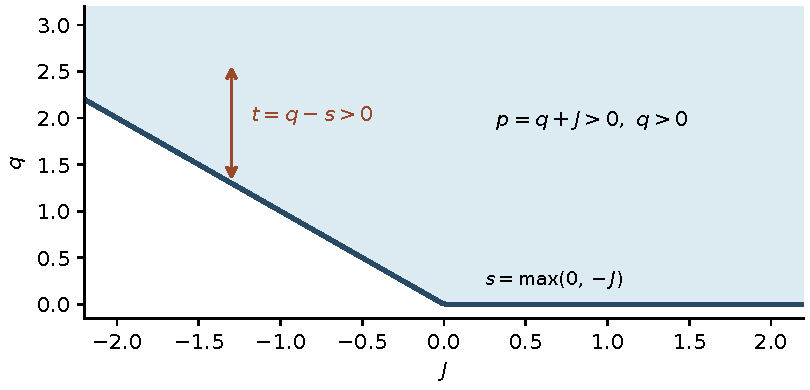
\includegraphics[width=.72\linewidth]{figures/admissibility.pdf}
\caption{One stationary-flow coordinate. Admissible reverse flows lie above the graph of $s=\max(0,-J)$; the parameter $t=q-s>0$ is the same on either side of $J=0$.}
\label{fig:admissibility}
\end{figure}

Set
\begin{equation}\label{eq:A}
A(e)=\diag\bigl(s(e)\bigr)-B(e).
\end{equation}
By~\eqref{eq:factor} and Lemma~\ref{lem:admissibility}, for admissible $(p,q)$ at degradation flux $e$,
\begin{equation}\label{eq:detH}
\det(-H)=(\det N)^2\det\bigl(A(e)+\diag(t)\bigr),\qquad t=\min(p,q)>0 .
\end{equation}
Proposition~\ref{prop:interior}(ii) therefore says exactly that for $e>0$,
\begin{equation}\label{eq:interiorA}
\det\bigl(A(e)+\diag(t)\bigr)\neq0\qquad\text{for every }t>0 .
\end{equation}

\subsection{Two lemmas on diagonal shifts}

\begin{lemma}[Orientation on the positive diagonal orthant]\label{lem:orientation}
Let $A$ be a real $n\times n$ matrix such that $\det(A+\diag(r))\neq0$ for every $r>0$. Then $\det(A+\diag(t))>0$ for every $t>0$.
\end{lemma}

\begin{proof}
For $\tau>0$ small, $\det(I+\tau A)>0$ by continuity, so $b=\tau^{-1}\one$ satisfies $\det(A+\diag(b))=\tau^{-n}\det(I+\tau A)>0$. The segment $r(\theta)=(1-\theta)b+\theta t$, $\theta\in[0,1]$, lies in the positive orthant, along which the determinant is continuous and never zero by hypothesis. By the intermediate value theorem it keeps the sign it has at $\theta=0$.
\end{proof}

\begin{lemma}[Strictness from nonnegativity]\label{lem:strict}
Let $A$ be a real $n\times n$ matrix such that $\det(A+\diag(r))\ge0$ for every $r>0$. Then $\det(A+\diag(t))>0$ for every $t>0$.
\end{lemma}

\begin{proof}
Fix $t>0$ and choose $a=t/2$ and $b>t$ so large coordinatewise that $A+\diag(b)$ is strictly diagonally dominant; then it is nonsingular~\cite[Theorem~6.1.10]{HJ13}, and its determinant, being nonnegative by hypothesis, is positive. The function $r\mapsto\det(A+\diag(r))$ is affine in each coordinate of $r$ separately. Hence its value at the interior point $t$ of the box $\prod_i[a_i,b_i]$ is the convex combination of its values at the $2^n$ vertices with the strictly positive weights $\prod_i\theta_i^{\epsilon_i}(1-\theta_i)^{1-\epsilon_i}$, $\theta_i=(b_i-t_i)/(b_i-a_i)\in(0,1)$. Every vertex value is nonnegative and the value at the vertex $b$ is positive.
\end{proof}

\subsection{The boundary theorem}

\begin{theorem}[Boundary nonsingularity]\label{thm:boundary}
Let $\ell\ge3$ and consider a separated Type $\II_\ell$ skeleton with positive integer active weights and unit terminal weights. For every $p,q>0$ and $e\ge0$ with $N(p-q)=e$, the matrix $H$ of~\eqref{eq:H} satisfies
\[
(-1)^n\det H=\det(-H)>0 .
\]
In particular, at every positive stationary state $x$ with arbitrary $d\ge0$, the physical Jacobian $D_xf(x)$ is nonsingular.
\end{theorem}

\begin{proof}
Let $e\ge0$ and $\varepsilon>0$, and put $e_\varepsilon=e+\varepsilon\one>0$. By~\eqref{eq:interiorA}, $A(e_\varepsilon)+\diag(r)$ is nonsingular for every $r>0$, so Lemma~\ref{lem:orientation} gives $\det(A(e_\varepsilon)+\diag(r))>0$ for all $r>0$. The maps $e\mapsto J=Ve$, $e\mapsto s(e)$ and $e\mapsto B(e)$ are continuous, hence so is $e\mapsto A(e)$, and letting $\varepsilon\downarrow0$ gives $\det(A(e)+\diag(r))\ge0$ for all $r>0$. Lemma~\ref{lem:strict} upgrades this to $\det(A(e)+\diag(t))>0$ for all $t>0$. By Lemma~\ref{lem:admissibility} the given $(p,q)$ correspond to $t=\min(p,q)>0$, and~\eqref{eq:detH} gives $\det(-H)>0$.

For the last statement, differentiate~\eqref{eq:model}: $\partial q_r/\partial x_i=q_rP_{ir}/x_i$, so
\begin{equation}\label{eq:physical}
D_xf(x)\,\diag(x)=N\diag(p)-N\diag(q)P^{\mathsf T}-\diag(e)=H
\end{equation}
with $(p,q,e)$ the flows of $x$, which satisfy $N(p-q)=e\ge0$.
\end{proof}

\begin{remark}
The proof uses interior nonsingularity at \emph{every} admissible flow triple $(p,q,e_\varepsilon)$, not merely along one family $(p_\varepsilon,q_\varepsilon,e_\varepsilon)$ converging to the given boundary triple. A single convergent family would only give $\det(A(e)+\diag(t))\ge0$ at one point $t$, from which nothing follows; it is the nonnegativity on the whole orthant that Lemma~\ref{lem:strict} converts into strict positivity. This is the uniform replacement for a case analysis over degradation supports: no enumeration of which coordinates of $d$ vanish is needed.
\end{remark}

\section{Type II: uniqueness transfer and the coincident branch}\label{sec:finish}

\subsection{Transfer from positive degradation}

\begin{lemma}[Boundary uniqueness transfer]\label{lem:ift}
Let $\Omega\subset\R^n$ be open and let $F$ be continuously differentiable on an open neighbourhood of $\{0\}\times\Omega$ in $\R\times\R^n$. Suppose that for every sufficiently small $\varepsilon>0$ the equation $F(\varepsilon,z)=0$ has at most one solution $z\in\Omega$, and that $D_zF(0,z)$ is invertible at every $z\in\Omega$ with $F(0,z)=0$. Then $F(0,z)=0$ has at most one solution in $\Omega$.
\end{lemma}

\begin{proof}
Let $x,y\in\Omega$ be zeros of $F(0,\cdot)$. By the implicit-function theorem~\cite{KP02} there are open intervals about $0$ and continuous branches $x(\varepsilon)$, $y(\varepsilon)$ with values in $\Omega$, $x(0)=x$, $y(0)=y$ and $F(\varepsilon,x(\varepsilon))=F(\varepsilon,y(\varepsilon))=0$. On the intersection of the two intervals, for every $\varepsilon>0$ small enough, interior uniqueness gives $x(\varepsilon)=y(\varepsilon)$. Letting $\varepsilon\downarrow0$ gives $x=y$.
\end{proof}

\begin{proof}[Proof of Theorem~\ref{thm:main}, separated Type $\II_\ell$ branch]
Fix the rate constants and $d\ge0$. Compress the return paths by Lemmas~\ref{lem:unit} and~\ref{lem:path}, so that two positive stationary states of the literal network give two positive stationary states of the skeleton at an effective nonnegative loss vector $d'\ge d$ (degradation plus path leakage). It suffices to identify the skeleton states; Lemma~\ref{lem:path} then identifies every internal path concentration.

Work in logarithmic coordinates $x=e^z$, $z\in\R^n$, and put
\[
F(\varepsilon,z)=N\bigl(a\odot e^{z}-b\odot e^{P^{\mathsf T}z}\bigr)-\diag(d'+\varepsilon\one)\,e^{z},
\]
where $\odot$ is the coordinatewise product and $e^{P^{\mathsf T}z}$ is the vector of monomials $\prod_ix_i^{P_{ir}}$. This is a smooth map on all of $\R\times\R^n$, and $F(\varepsilon,z)=0$ if and only if $x=e^z$ is a positive stationary state of the skeleton at degradation $d'+\varepsilon\one$; only $\varepsilon\ge0$ is physical, but the map makes sense for all real $\varepsilon$. For every $\varepsilon>0$ the degradation vector $d'+\varepsilon\one$ is strictly positive, so Proposition~\ref{prop:interior}(i) gives at most one zero. At a zero of $F(0,\cdot)$, the derivative $D_zF(0,z)$ is exactly the matrix $H$ of~\eqref{eq:H} with the flows of $x=e^z$ at degradation $d'$, which is invertible by Theorem~\ref{thm:boundary}. Lemma~\ref{lem:ift} with $\Omega=\R^n$ gives uniqueness.
\end{proof}

The proof does not assume that a positive stationary state exists at any parameter, nor that the branches can be continued globally; the continuation is local around each hypothetical root and uses the same positive perturbation of all losses simultaneously.

\subsection{The coincident three-fork branch}
It remains to treat the exceptional network~\eqref{eq:coincident} of Lemma~\ref{lem:exhaustion}, with currents $J_i(x)=a_ix_i-b_ix_{i+1}^{m_i}x_{i+2}$ and stationary equations $NJ=\diag(d)x$, where, in the order $0,1,2$,
\[
N=\begin{pmatrix}-1&1&m_2\\ m_0&-1&1\\ 1&m_1&-1\end{pmatrix},\qquad
\det N=m_0+m_1+m_2+m_0m_1m_2>0 .
\]
The inverse $V=N^{-1}$ has strictly positive off-diagonal entries:
\begin{equation}\label{eq:inverse}
(\det N)\,V=\begin{pmatrix}
1-m_1&1+m_1m_2&1+m_2\\
1+m_0&1-m_2&1+m_0m_2\\
1+m_0m_1&1+m_1&1-m_0
\end{pmatrix}.
\end{equation}

\begin{proposition}[Coincident branch]\label{prop:coincident}
For positive rate constants, positive integer weights $m_i$ and $d\ge0$, the network~\eqref{eq:coincident} has at most one positive stationary state.
\end{proposition}

\begin{proof}
Let $x,y>0$ be stationary and put $r_i=x_i/y_i$. From $J(x)=V\diag(d)x$ and $J(y)=V\diag(d)y$, the cross combination $x_iJ_i(y)-y_iJ_i(x)$ has vanishing diagonal term and equals
\begin{equation}\label{eq:weightedcross}
x_iJ_i(y)-y_iJ_i(x)=\sum_{j\ne i}V_{ij}d_j\,(x_iy_j-y_ix_j)=\sum_{j\neq i}V_{ij}d_j\,y_iy_j\,(r_i-r_j).
\end{equation}
From the mass-action form of the currents the same quantity equals
\begin{equation}\label{eq:crossleft}
b_i\,y_iy_{i+1}^{m_i}y_{i+2}\,\bigl(r_{i+1}^{m_i}r_{i+2}-r_i\bigr).
\end{equation}
If all three ratios equal $r$, the right side of~\eqref{eq:weightedcross} vanishes, so $r^{m_i+1}=r$ and $r=1$. Otherwise write the ordered ratios as $0<L\le M\le H$ with $L<H$. At an index where $r_i=H$ the right side of~\eqref{eq:weightedcross} is nonnegative, since $V_{ij}>0$, $d_j\ge0$ and $r_i\ge r_j$; at an index where $r_i=L$ it is nonpositive. We show that one of the two corresponding left sides~\eqref{eq:crossleft} has the strictly opposite sign. Depending on the cyclic position of the maximum, the two tests are, with exponents $a,b\ge1$,
\[
L^aM<H\ \text{ or }\ M^bH>L,
\qquad\text{or}\qquad
M^aL<H\ \text{ or }\ H^bM>L .
\]
In the first pair, if $L^aM\ge H$ then $L^a\ge H/M\ge1$, so $L\ge1$, $M\ge1$ and $M^bH\ge H>L$. In the second pair, if $H^bM\le L$ then $H^b\le L/M\le1$, so $H\le1$, $M\le1$ and $M^aL\le L<H$. In either case one strict sign contradiction occurs. Hence $r\equiv1$.
\end{proof}

By Lemma~\ref{lem:exhaustion}, the separated and coincident branches exhaust the source-minimal Type $\II_\ell$ cores with $\ell\ge3$. Together with Section~\ref{sec:typev}, this completes the proof of Theorem~\ref{thm:main}. \qed

\section{Consequences}\label{sec:consequences}

The results of this section are conventional consequences of Theorems~\ref{thm:main} and~\ref{thm:boundary}; they are not part of the formal development except where indicated.

\subsection{A quantitative determinant bound}

\begin{lemma}[Diagonal-shift bound]\label{lem:bound}
Let $A\in\R^{n\times n}$ satisfy $\det(A+\diag(r))\ge0$ for every $r>0$. Then every principal minor of $A$ is nonnegative, and
\begin{equation}\label{eq:bound}
\det\bigl(A+\diag(t)\bigr)\ \ge\ \prod_{i=1}^nt_i\qquad(t\ge0).
\end{equation}
\end{lemma}

\begin{proof}
Recall the expansion $\det(A+\diag(r))=\sum_{S}\det A[S]\prod_{i\notin S}r_i$ over subsets $S\subseteq\{1,\dots,n\}$, where $A[S]$ is the principal submatrix on $S$ and the empty minor equals one. Fix $S$ and $\varepsilon>0$, and put $r_i=\varepsilon$ for $i\in S$, $r_i=T$ for $i\notin S$. As a polynomial in $T$ the determinant has degree at most $n-|S|$, and the coefficient of $T^{n-|S|}$ is $\sum_{S'\subseteq S}\det A[S']\,\varepsilon^{|S\setminus S'|}=\det(A[S]+\varepsilon I_S)$. Dividing the hypothesis by $T^{n-|S|}$ and letting $T\to\infty$ gives $\det(A[S]+\varepsilon I_S)\ge0$; letting $\varepsilon\downarrow0$ gives $\det A[S]\ge0$. In the expansion at $t\ge0$ every summand is then nonnegative, and the summand for $S=\varnothing$ is $\prod_it_i$.
\end{proof}

\begin{corollary}[Stationary determinant bound]\label{cor:bound}
In the setting of Theorem~\ref{thm:boundary}, for every $p,q>0$ and $e\ge0$ with $N(p-q)=e$,
\begin{equation}\label{eq:chemical}
\det(-H)\ \ge\ (\det N)^2\prod_i\min\{p_i,q_i\}\ >0,
\end{equation}
and at a positive stationary state $x$, $\det(-D_xf(x))\ge(\det N)^2\prod_i\min\{p_i,q_i\}/\prod_ix_i$.
\end{corollary}

\begin{proof}
The proof of Theorem~\ref{thm:boundary} established the hypothesis of Lemma~\ref{lem:bound} for $A(e)$; combine~\eqref{eq:bound} with~\eqref{eq:detH}, Lemma~\ref{lem:admissibility} and~\eqref{eq:physical}.
\end{proof}

The bound is stated for the retained separated skeleton; no bound is claimed for the expanded network with return paths, for the coincident branch, or for the condition number. A lower bound on a determinant is not a lower bound on the smallest singular value.

\subsection{Local continuation}
Theorem~\ref{thm:boundary} and Proposition~\ref{prop:tangent} (lifted through the Schur complement of the eliminated path and fork-source species, whose blocks are invertible by the passive-chain energy identity of Remark~\ref{rem:lift}) give nonsingularity of the physical Jacobian at every positive stationary state of both families, for all rate constants and all $d\ge0$. The implicit-function theorem in all parameters then gives a locally smooth stationary branch through every positive stationary state, which stays positive and, restricted to $d\ge0$, coincides by Theorem~\ref{thm:main} with the unique positive state at each nearby parameter. Consequently, turning an individual loss coefficient through zero cannot produce a local ambiguity between two positive branches, and no interior saddle-node bifurcation of positive states can occur while the hypotheses hold. Global continuation would additionally require the branch to stay in a compact subset of the positive orthant; nothing here excludes escape to the boundary or to infinity, nor a Hopf bifurcation, and nonsingularity does not by itself imply attraction.

\begin{remark}[The physical Jacobian of Type $\V$]\label{rem:lift}
After path compression the three fork-source equations $a_iU_i-D_iS_i+g_iW_i=0$ have a diagonal derivative block $-\diag(D_i)$ in $S$. Eliminating $S$ leaves the three pair balances $E_i=\delta_{i+1}+\delta_{i+2}-\delta_i-L_i$, and with $Q=\one\one^{\mathsf T}-2I$ one has $E=Q\delta-L$, $\det Q=4$. The row transformation $R=2Q^{-1}E=2\delta-(\one\one^{\mathsf T}-I)L$ satisfies $R_i=U_i(2\alpha_i-G_i(U))$ at a root, so $DR=-\diag(U)\,DG(U)$ there, which is nonsingular by Proposition~\ref{prop:tangent}. For the internal species of a unit path, with the detailed-balance weights $\pi_0>0$, $\pi_{k+1}=a_k\pi_k/b_k$ and $c_k=a_k\pi_k$, a homogeneous perturbation $y_k=\pi_kz_k$ with $z_0=z_{m+1}=0$ satisfies the energy identity
\[
-\sum_{k=1}^mz_k\,(\mathcal Ly)_k=\sum_{k=0}^mc_k(z_{k+1}-z_k)^2+\sum_{k=1}^md_k\pi_kz_k^2,
\]
where $\mathcal L$ is the internal Jacobian of the path; so $\mathcal L$ is invertible even when every internal loss vanishes. Block elimination then lifts nonsingularity from the reduced system to the literal network, $\det\mathcal J=\det\mathcal L\cdot\det Df_{\mathrm{red}}$. The same tangent row, with $b=B_i$, $c=C_i$, $d=D_i$, $h=0$ and $k=B_i(m_i-1)\ge0$, covers the coincident Type $\II_3$ branch, using the positive off-diagonal entries of~\eqref{eq:inverse}. These derivative identifications are conventional; only the algebraic kernel criterion of Proposition~\ref{prop:tangent} is formalized.
\end{remark}

\subsection{Small degradation: existence and stability}

\begin{proposition}[Small degradation]\label{prop:small}
Fix a source-minimal Type $\II_\ell$ core with $\ell\ge3$ or a Type $\V$ core, with its unit paths, and fix positive reversible rate constants. There is a neighbourhood of $d=0$ in $\R^n$ such that every nonnegative degradation vector in it admits exactly one positive stationary state, and this state is locally asymptotically stable.
\end{proposition}

\begin{proof}
Every species of the literal network is the reactant of exactly one reaction, so $N$ is square, and it is invertible. Indeed, $NJ=0$ forces equal currents along every unit path, so it suffices to check the collapsed skeletons: Lemma~\ref{lem:invertible} covers the separated Type $\II_\ell$ case, $\det N>0$ covers the coincident one, and for Type $\V$ the balances at $S_i$ and $U_i$ give $\delta_{i+1}+\delta_{i+2}=\delta_i$ for the three fork currents, whence $\sum_i\delta_i=0$ and then $\delta=0$. At $d=0$ stationarity reads $N(p-q)=0$, hence $p=q$: every reaction is individually balanced. Taking logarithms, $p=q$ is the linear system $N^{\mathsf T}\log x=\log(a/b)$, which has a unique solution $\log x^*$, so there is exactly one positive stationary state $x^*$, and it is detailed balanced in the sense of Horn and Jackson~\cite{HJ72}. Put $X=\diag(x^*)$ and $Q=\diag(q^*)>0$. By~\eqref{eq:physical} with $p=q$ and $e=0$, the physical Jacobian is $\mathcal J_0=-NQN^{\mathsf T}X^{-1}$, which is similar to $-X^{-1/2}NQN^{\mathsf T}X^{-1/2}$; this is symmetric and negative definite, since $v^{\mathsf T}X^{-1/2}NQN^{\mathsf T}X^{-1/2}v=\|Q^{1/2}N^{\mathsf T}X^{-1/2}v\|^2>0$ for $v\ne0$ by invertibility of $N$. The implicit-function theorem gives a positive stationary state for all $d$ near $0$, depending smoothly on $d$, and by openness of the Hurwitz condition its Jacobian has all eigenvalues in the open left half plane for $d$ small; local asymptotic stability follows from the linearization theorem for smooth finite-dimensional dynamics. Theorem~\ref{thm:main} makes it the only positive stationary state. The neighbourhood depends on the network and its rates but contains small nonnegative vectors of every support.
\end{proof}

\subsection{Nonnegative stationary states}

\begin{proposition}[Origin or positive]\label{prop:boundarystates}
A nonnegative stationary state of the reversible extension of a diluted core, with nonnegative linear degradation, is either the origin or strictly positive. Hence such a network has at most two nonnegative stationary states, the origin and possibly one positive state.
\end{proposition}

\begin{proof}
Suppose $x\ge0$ is stationary and $x_i=0$. In the balance of $X_i$, the consumption terms (forward consumption $a_ix_i$, reverse consumption of the reactions producing $X_i$, and degradation) all vanish, so the remaining production terms, which are nonnegative, sum to zero and therefore each vanish. For every forward reaction $r$ with $P_{ir}>0$, its forward production $a_rP_{ir}x_r$ vanishes, so $x_r=0$. Thus a zero propagates backward along every edge $X_r\to X_i$ of the split graph; since the split graph of a core is strongly connected, $x=0$. Conversely the origin is stationary, since every reaction has a reactant among the species and degradation is linear. The count follows from Corollary~\ref{cor:classification}.
\end{proof}

\section{Formal verification}\label{sec:formal}

The two families of Theorem~\ref{thm:main} are compiled in Lean~4~\cite{dMU21}, version~4.30.0, against a frozen Mathlib~\cite{mathlib20} manifest with SHA-256
\begin{center}\small\texttt{a8df0b606ec258561c226df89856884be433c19b49fb0a27335d69bb2b6e9fac}.\end{center}
The terminal declaration, in the namespace \lean{MixedDegradation}, is
\begin{lstlisting}
theorem paper_mixed_degradation_unistationarity :
    (∀ (l : ℕ) (Q : TypeII.PaperRaw.OpenNetwork l),
      TypeII.PaperRaw.IsPaperTypeIILCore Q → 3 ≤ l →
      ∀ x y : Q.State, Q.PositiveState x → Q.PositiveState y →
        Q.Stationary x → Q.Stationary y → x = y) ∧
    (∀ (N : TypeV.Network) (x y : TypeV.State N),
      TypeV.PositiveState N x → TypeV.PositiveState N y →
        TypeV.Stationary N x → TypeV.Stationary N y → x = y)
\end{lstlisting}
It is an independent conjunction of two universal statements: neither conjunct is used in the proof of the other, and neither has an outer hypothesis beyond its own network and states.

\subsection*{The Type II interface}
\lean{OpenNetwork l} is the literal weak-order source normal form of Section~\ref{subsec:typeii}, inherited from~\cite{TypeIIpos}: a Boolean weak-stem word, a separated realization with cyclic source partition, arbitrary positive integer main weights, coefficient-one back products, common positive rate constants, and literal reversible unit return chains, together with the data of the coincident three-fork quotient. The only change from the positive-degradation development is the rate record, which now carries \emph{nonnegative} degradation constants for every retained and every internal species. \lean{IsPaperTypeIILCore Q} consists of $\Top$ and source minimality, in the form that no proper weak-stem restriction retains $\Top$ and no rotated proper return cycle is stoichiometrically autocatalytic. \lean{State}, \lean{PositiveState} and \lean{Stationary} select the literal concentration space and the finite mass-action balance equations of the active branch, including every internal return-chain species. Lemma~\ref{lem:exhaustion} is the inherited declaration \lean{source_exhaustion_of_minimal}; Lemma~\ref{lem:unit} is derived inside the family proof from the minimality predicate.

\subsection*{The Type V interface}
\lean{TypeV.Network} consists of three sectors, each either \lean{collapsed} or \lean{linked} with an arbitrary finite \lean{UnitChain} and a nonnegative loss at the fork source, together with positive forward and reverse fork constants and nonnegative base losses. \lean{TypeV.State N} contains the three base concentrations and, for each linked sector, the fork-source concentration and the full chain state. \lean{Stationary} is the literal set of balances at every base, fork-source and internal species; \lean{PositiveState} requires positivity of every one of these concentrations. All eight identification patterns and all chain lengths are instances of a single parametric proof.

\subsection*{Module map}
Table~\ref{tab:modules} lists the correspondence between the arguments of this paper and the formal modules under \lean{proofs/MixedDegradation/}. The general determinant lemmas of Section~\ref{sec:boundary} are stated for arbitrary finite index types; the boundary theorem instantiates them on the source stoichiometric matrix. The uniqueness transfer uses Mathlib's implicit-function theorem for maps with product domain, applied to the logarithmic drift $F(\varepsilon,z)$ of Section~\ref{sec:finish}, whose strict Fr\'echet derivative is computed in \lean{LogDrift.lean}; \lean{TypeIISkeleton.lean} converts the exponential coordinates back to the literal integer-power monomials of the source model.

\begin{table}[H]
\centering\small
\begin{tabular}{>{\raggedright\arraybackslash}p{.30\linewidth}>{\raggedright\arraybackslash}p{.64\linewidth}}
\toprule
Statement in this paper & Formal modules and principal declarations\\
\midrule
Lemma~\ref{lem:path}, passive paths with nonnegative loss & \lean{PassiveChain.lean}: \lean{chain_flux_compress}, \lean{chain_state_unique}\\
Lemma~\ref{lem:ratios} and the Type V family theorem & \lean{TypeVReduced.lean}: \lean{side_extremum}, \lean{rowDefect_pos}, \lean{rowDefect_neg}, \lean{reduced_unistationarity}; \lean{TypeVSource.lean}: \lean{paper_type_v_unistationarity}\\
Proposition~\ref{prop:tangent}, tangent kernel & \lean{TypeVDerivative.lean}: \lean{tangent_kernel_zero}; \lean{Publication.lean}: \lean{tangentMatrix_nonsingular}\\
Proposition~\ref{prop:interior}, one-state current criterion & \lean{TypeIIInterior.lean}: \lean{typeII_interior_current_kernel_nonsingular}, over the inherited \lean{TypeIIL} modules\\
Secant at $\rho=\one$; Sylvester bridge to $H$ & \lean{SourceSecantDerivative.lean}, \lean{CurrentJacobian.lean}, \lean{SourceJacobian.lean}\\
Lemma~\ref{lem:invertible} & \lean{SourceInvertible.lean}: \lean{typeII_source_stoich_nonsingular}\\
Factorization~\eqref{eq:factor} & \lean{StationaryJacobian.lean}: \lean{stationary_factorization}, \lean{stationary_signed_determinant}\\
Lemmas~\ref{lem:orientation} and~\ref{lem:strict} & \lean{InteriorBoundary.lean}: \lean{det_pos_of_nonsingular_diagonal_shifts}; \lean{DiagonalBoundary.lean}: \lean{det_pos_of_nonnegative_diagonal_shifts}\\
Theorem~\ref{thm:boundary} & \lean{StationaryBoundary.lean}: \lean{stationary_boundary_nonsingular}; \lean{SourceBoundary.lean}: \lean{typeII_boundary_jacobian_nonsingular}\\
Lemma~\ref{lem:ift} and the skeleton theorem & \lean{BoundaryUniqueness.lean}: \lean{boundary_uniqueness_of_nondegenerate}; \lean{LogDrift.lean}; \lean{TypeIISkeleton.lean}: \lean{typeII_skeleton_unistationarity}\\
Path compression and full-state join & \lean{TypeIILift.lean}: \lean{separated_unistationarity}; \lean{TypeIISource.lean}: \lean{paper_typeII_l_unistationarity}\\
Proposition~\ref{prop:coincident} & \lean{Coincident.lean}: \lean{all_zero_unistationarity}\\
Theorem~\ref{thm:main} & \lean{Main.lean}: \lean{paper_mixed_degradation_unistationarity}\\
\bottomrule
\end{tabular}
\caption{Correspondence between the paper and the Lean development. The historical name \texttt{all\_zero\_unistationarity} refers to the all-coincident stem word, not to zero degradation.}
\label{tab:modules}
\end{table}

\subsection*{Verification receipts}
The development was checked with warnings treated as errors and exit code zero. The receipt for \lean{Main.lean} (source SHA-256 \texttt{2a52e632\ldots7e7}) covers its complete closure of 88 local modules; the receipt for \lean{Publication.lean} (source SHA-256 \texttt{c9655673\ldots03}) covers 90 modules and exports both the terminal declaration and \lean{tangentMatrix_nonsingular}. The authenticated elaborated type of the terminal declaration has fingerprint
\begin{center}\small\texttt{sha256:90dc869ae55cb7a3319c015897ef5108667502803c00d00067b95bf5efa896de}.\end{center}
Both exported declarations report exactly the axioms \texttt{propext}, \texttt{Classical.choice} and \texttt{Quot.sound}, the standard foundation of Mathlib; there is no \texttt{sorry}, no native-computation axiom, and no assumed determinant, uniqueness or continuation certificate in any public interface.

\subsection*{What is and is not formal}
The following are formal: both family uniqueness theorems over the literal source normal forms; the passive-path reduction with nonnegative loss; the three-ratio and tangent-kernel criteria; the stationary factorization; the two diagonal-orthant determinant lemmas; the boundary nonsingularity of the retained skeleton; and the implicit-function transfer. The following are conventional mathematics in this paper: the identification of the source normal forms with the prose classification of~\cite{NNU26}, the five-family Corollary~\ref{cor:classification}, and the consequences of Section~\ref{sec:consequences}, including the derivative identifications of Remark~\ref{rem:lift} and the stability statement of Proposition~\ref{prop:small}. The exact rational stationary examples used as regression tests during development (ten models, including two with loss only at an internal path species and eight covering every Type $\V$ identification pattern at singleton loss support) are diagnostics, not premises.

\section{Discussion}\label{sec:discussion}

\subsection*{Relation to injectivity criteria}
Uniqueness of positive equilibria in mass-action systems is classically approached through injectivity of the species-formation rate function, certified by parameter-independent sign conditions on the Jacobian or on its minors: the injectivity property of Craciun and Feinberg~\cite{CF05,CF06}, its graph-theoretic forms~\cite{BC10}, the preclusion results of Feliu and Wiuf~\cite{FW12}, the sign conditions of M\"uller et al.~\cite{MFRCSD16}, and the surveys~\cite{JS15,Fei19}; parameter regions for multistationarity are studied in~\cite{CFMW17}. Such criteria cannot apply here: as shown in~\cite{TypeIIpos}, the minimal Type $\II_3$ wiring shares its sign pattern with nonminimal networks that are genuinely multistationary, and its logarithmically scaled Jacobian has a negative principal minor at some positive coefficient vectors that violate the stationary balance. The present argument is parameter-dependent in an explicit way: Proposition~\ref{prop:interior}(ii) and Theorem~\ref{thm:boundary} hold only on the stationary manifold $N(p-q)=e$, and Lemma~\ref{lem:bound} shows that on that manifold the matrix $A(e)$ is a $P_0$-matrix, so that $\diag(q)-B(e)$ is a $P$-matrix whenever $q$ is admissible. The classical theory of $P$-matrices explains why this suffices for nonsingularity; the content of the paper is that stationarity forces the $P_0$ property, uniformly in the degradation support.

\subsection*{Detailed balance and deficiency}
At $d=0$ the reversible extension of a core with invertible source matrix is detailed balanced, with the unique positive equilibrium of Proposition~\ref{prop:small}; this is the situation of Horn and Jackson~\cite{HJ72} and of the deficiency theorems of Feinberg~\cite{Fei87,Fei19}. Linear degradation destroys detailed balance and the complex-balanced structure, and the classical theorems no longer apply. Theorem~\ref{thm:main} may be read as the statement that, for the minimal cores, uniqueness of the positive state survives this loss of structure along every ray $d\ge0$, and Proposition~\ref{prop:small} shows that the equilibrium and its stability survive at least for small $d$. Whether the unique positive state is stable for all $d$, and whether it attracts all positive trajectories, is not addressed by our methods.

\subsection*{Open directions}
Three questions remain. First, existence: Theorem~\ref{thm:main} is an at-most-one statement, and the threshold in $d$ beyond which the positive state disappears (Proposition~\ref{prop:boundarystates} shows it must disappear into the origin or at infinity, not by collision with another positive state) is not characterized. Second, stability and oscillations: nonsingularity excludes saddle-nodes but not Hopf bifurcations, and the sign of the real parts of the eigenvalues of $H$ for large mixed degradation is open. Third, composition: the exact examples of~\cite{TypeIIpos} show that a nonminimal network built from a core and an embedded gain cycle can be multistationary already with positive degradation. The determinant identity~\eqref{eq:factor} and the admissibility shift apply verbatim to any network with a square invertible source matrix, and it would be interesting to know which composite networks of several interacting cores inherit the $P_0$ property of $A(e)$ on the stationary manifold.

\section*{Acknowledgements}
To be inserted.

\bibliographystyle{plain}
\bibliography{refs}

\end{document}
